\documentclass[10pt]{article}

\usepackage{amsmath}

\newcommand{\myvec}[1]{\ensuremath{\begin{pmatrix}#1\end{pmatrix}}}

\newcommand{\mydet}[1]{\ensuremath{\begin{vmatrix}#1\end{vmatrix}}}

\newcommand{\solution}{\noindent \textbf{Solution: }}

\providecommand{\brak}[1]{\ensuremath{\left(#1\right)}}

\providecommand{\norm}[1]{\left\lVert#1\right\rVert}
\usepackage{graphicx}
\usepackage{float}
\let\vec\mathbf
\title{Coordinate Geometry}
\author{Divyanshu Sharma (divyansusharma@sriprakashschools.com)}

\begin{document}
\maketitle
\section*{Class 10$^{th}$ Maths - Chapter 7}
This is Problem-1(ii) from Exercise 7.3
\begin{enumerate}
\item Find the area of the triangle whose vertices are:
\begin{align}
{(-5,-1),(3,-5),(5,2)}
\end{align}
\solution \\
Given Data:
\begin{align}
\vec{A} &= \myvec{-5\\-1}\\
\vec{B} &= \myvec{3\\-5}\\
\vec{C} &= \myvec{5\\2}\\
\end{align}
\begin{align}
\vec{AB} &= \myvec{8\\-4}\\
\vec{AC} &= \myvec{10\\3}\\
\end{align}
AREA OF THE TRIANGLE:
\begin{align}
\\&=\frac{1}{2}\norm{{\vec{AB}}\times \vec{AC}}\\
\\&=\frac{1}{2}\mydet{8 & 10 \\ -4 & 3}\\
\\&=\frac{1}{2}\norm{24+40}\\
\\&=\frac{1}{2}\norm{64}\\
\\&= {32} sq.units
\end{align}
\end{enumerate}
\begin{figure}[H]
			\centering
			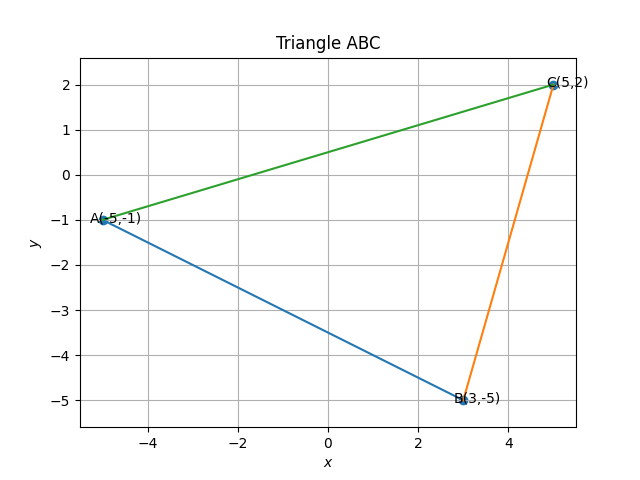
\includegraphics[width=\columnwidth]{figs/Figure_1.png}
			\caption{Triangle ABC}
			\label{fig:txn1}
		\end{figure}
\end{document}

